\begin{figure*}[t]
\centering
\resizebox{\textwidth}{!}{%
  % Generated by scripts/figures/generate_main_matrix_host_latency_tikz.py.
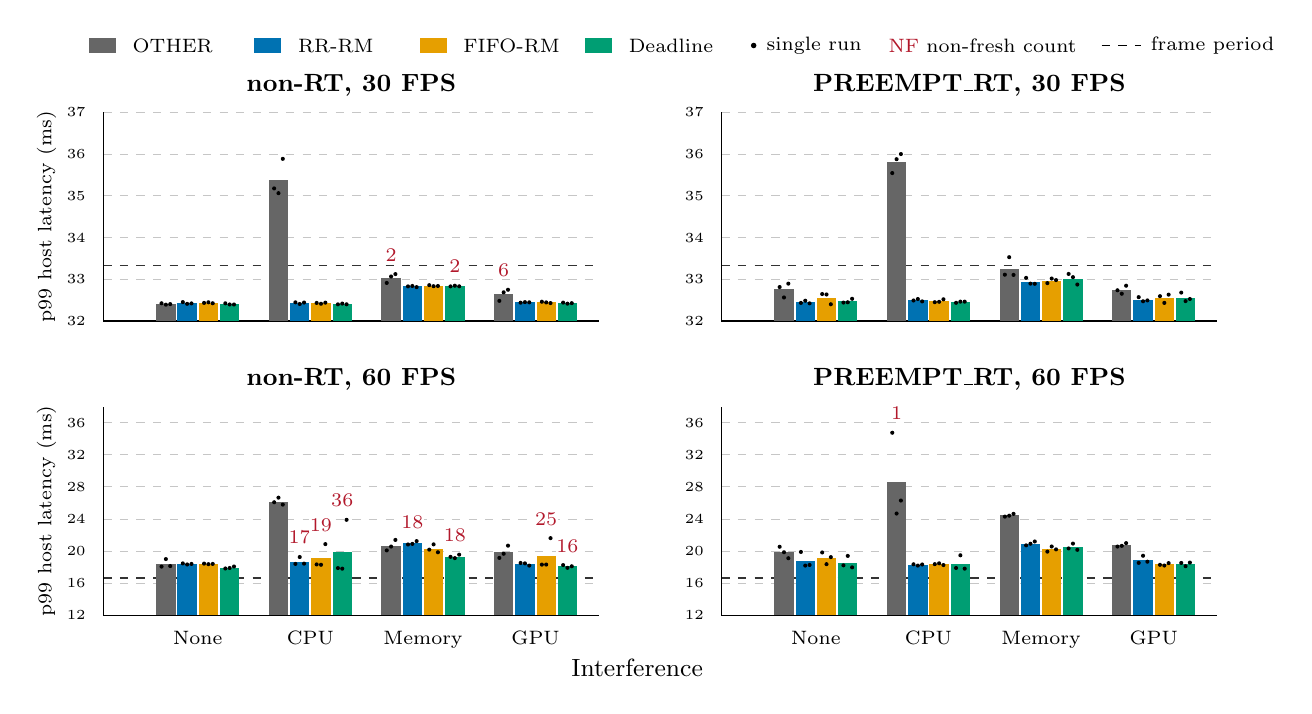
\begin{tikzpicture}[x=1cm,y=1cm,font=\scriptsize]
  \definecolor{pOneOther}{HTML}{666666}
  \definecolor{pOneRr}{HTML}{0072B2}
  \definecolor{pOneFifo}{HTML}{E69F00}
  \definecolor{pOneDeadline}{HTML}{009E73}
  \definecolor{pOneNonFresh}{HTML}{B2182B}
  \fill[pOneOther] (1.42,8.54) rectangle ++(0.34,0.18);
  \node[anchor=west] at (1.85,8.63) {OTHER};
  \fill[pOneRr] (3.52,8.54) rectangle ++(0.34,0.18);
  \node[anchor=west] at (3.95,8.63) {RR-RM};
  \fill[pOneFifo] (5.62,8.54) rectangle ++(0.34,0.18);
  \node[anchor=west] at (6.05,8.63) {FIFO-RM};
  \fill[pOneDeadline] (7.72,8.54) rectangle ++(0.34,0.18);
  \node[anchor=west] at (8.15,8.63) {Deadline};
  \fill[black] (9.86,8.63) circle (0.035);
  \node[anchor=west] at (9.90,8.63) {single run};
  \node[text=pOneNonFresh,anchor=west] at (11.45,8.63) {NF};
  \node[anchor=west] at (11.93,8.63) {non-fresh count};
  \draw[dashed,line width=0.45pt] (14.28,8.63)--(14.78,8.63);
  \node[anchor=west] at (14.78,8.63) {frame period};
  \node[font=\small\bfseries] at (4.75,8.13) {non-RT, 30 FPS};
  \draw[gray!45,dashed,line width=0.35pt] (1.6,5.13)--(7.9,5.13);
  \node[anchor=east,font=\tiny] at (1.5,5.13) {32};
  \draw[gray!45,dashed,line width=0.35pt] (1.6,5.66)--(7.9,5.66);
  \node[anchor=east,font=\tiny] at (1.5,5.66) {33};
  \draw[gray!45,dashed,line width=0.35pt] (1.6,6.19)--(7.9,6.19);
  \node[anchor=east,font=\tiny] at (1.5,6.19) {34};
  \draw[gray!45,dashed,line width=0.35pt] (1.6,6.72)--(7.9,6.72);
  \node[anchor=east,font=\tiny] at (1.5,6.72) {35};
  \draw[gray!45,dashed,line width=0.35pt] (1.6,7.25)--(7.9,7.25);
  \node[anchor=east,font=\tiny] at (1.5,7.25) {36};
  \draw[gray!45,dashed,line width=0.35pt] (1.6,7.78)--(7.9,7.78);
  \node[anchor=east,font=\tiny] at (1.5,7.78) {37};
  \draw[black!80,dashed,line width=0.55pt] (1.6,5.8367)--(7.9,5.8367);
  \draw[line width=0.45pt] (1.6,5.13)--(7.9,5.13);
  \draw[line width=0.45pt] (1.6,5.13)--(1.6,7.78);
  \fill[pOneOther] (2.2725,5.13) rectangle (2.5175,5.3469);
  \fill[black] (2.34,5.3564) circle (0.026);
  \fill[black] (2.395,5.3384) circle (0.026);
  \fill[black] (2.45,5.3458) circle (0.026);
  \fill[pOneRr] (2.5425,5.13) rectangle (2.7875,5.3584);
  \fill[black] (2.61,5.3712) circle (0.026);
  \fill[black] (2.665,5.3492) circle (0.026);
  \fill[black] (2.72,5.3547) circle (0.026);
  \fill[pOneFifo] (2.8125,5.13) rectangle (3.0575,5.3623);
  \fill[black] (2.88,5.3611) circle (0.026);
  \fill[black] (2.935,5.3691) circle (0.026);
  \fill[black] (2.99,5.3567) circle (0.026);
  \fill[pOneDeadline] (3.0825,5.13) rectangle (3.3275,5.3459);
  \fill[black] (3.15,5.3559) circle (0.026);
  \fill[black] (3.205,5.3411) circle (0.026);
  \fill[black] (3.26,5.3407) circle (0.026);
  \fill[pOneOther] (3.7025,5.13) rectangle (3.9475,6.9201);
  \fill[black] (3.77,6.815) circle (0.026);
  \fill[black] (3.825,6.7546) circle (0.026);
  \fill[black] (3.88,7.1906) circle (0.026);
  \fill[pOneRr] (3.9725,5.13) rectangle (4.2175,5.3604);
  \fill[black] (4.04,5.3684) circle (0.026);
  \fill[black] (4.095,5.3473) circle (0.026);
  \fill[black] (4.15,5.3656) circle (0.026);
  \fill[pOneFifo] (4.2425,5.13) rectangle (4.4875,5.3585);
  \fill[black] (4.31,5.3605) circle (0.026);
  \fill[black] (4.365,5.3504) circle (0.026);
  \fill[black] (4.42,5.3644) circle (0.026);
  \fill[pOneDeadline] (4.5125,5.13) rectangle (4.7575,5.3464);
  \fill[black] (4.58,5.3431) circle (0.026);
  \fill[black] (4.635,5.3526) circle (0.026);
  \fill[black] (4.69,5.3434) circle (0.026);
  \fill[pOneOther] (5.1325,5.13) rectangle (5.3775,5.6794);
  \fill[black] (5.2,5.6147) circle (0.026);
  \fill[black] (5.255,5.6964) circle (0.026);
  \fill[black] (5.31,5.7271) circle (0.026);
  \node[text=pOneNonFresh,font=\scriptsize,fill=white,inner sep=0.25pt,anchor=south] at (5.255,5.8771) {2};
  \fill[pOneRr] (5.4025,5.13) rectangle (5.6475,5.5695);
  \fill[black] (5.47,5.5709) circle (0.026);
  \fill[black] (5.525,5.576) circle (0.026);
  \fill[black] (5.58,5.5615) circle (0.026);
  \fill[pOneFifo] (5.6725,5.13) rectangle (5.9175,5.5785);
  \fill[black] (5.74,5.5866) circle (0.026);
  \fill[black] (5.795,5.5732) circle (0.026);
  \fill[black] (5.85,5.5757) circle (0.026);
  \fill[pOneDeadline] (5.9425,5.13) rectangle (6.1875,5.5741);
  \fill[black] (6.01,5.5709) circle (0.026);
  \fill[black] (6.065,5.5792) circle (0.026);
  \fill[black] (6.12,5.5721) circle (0.026);
  \node[text=pOneNonFresh,font=\scriptsize,fill=white,inner sep=0.25pt,anchor=south] at (6.065,5.7292) {2};
  \fill[pOneOther] (6.5625,5.13) rectangle (6.8075,5.4702);
  \fill[black] (6.63,5.387) circle (0.026);
  \fill[black] (6.685,5.4956) circle (0.026);
  \fill[black] (6.74,5.5279) circle (0.026);
  \node[text=pOneNonFresh,font=\scriptsize,fill=white,inner sep=0.25pt,anchor=south] at (6.685,5.6779) {6};
  \fill[pOneRr] (6.8325,5.13) rectangle (7.0775,5.3676);
  \fill[black] (6.9,5.3638) circle (0.026);
  \fill[black] (6.955,5.3708) circle (0.026);
  \fill[black] (7.01,5.3683) circle (0.026);
  \fill[pOneFifo] (7.1025,5.13) rectangle (7.3475,5.3674);
  \fill[black] (7.17,5.3758) circle (0.026);
  \fill[black] (7.225,5.3674) circle (0.026);
  \fill[black] (7.28,5.359) circle (0.026);
  \fill[pOneDeadline] (7.3725,5.13) rectangle (7.6175,5.3582);
  \fill[black] (7.44,5.3653) circle (0.026);
  \fill[black] (7.495,5.3514) circle (0.026);
  \fill[black] (7.55,5.3577) circle (0.026);
  \node[rotate=90,font=\scriptsize] at (0.88,6.455) {p99 host latency (ms)};
  \node[font=\small\bfseries] at (12.6,8.13) {PREEMPT\_RT, 30 FPS};
  \draw[gray!45,dashed,line width=0.35pt] (9.45,5.13)--(15.75,5.13);
  \node[anchor=east,font=\tiny] at (9.35,5.13) {32};
  \draw[gray!45,dashed,line width=0.35pt] (9.45,5.66)--(15.75,5.66);
  \node[anchor=east,font=\tiny] at (9.35,5.66) {33};
  \draw[gray!45,dashed,line width=0.35pt] (9.45,6.19)--(15.75,6.19);
  \node[anchor=east,font=\tiny] at (9.35,6.19) {34};
  \draw[gray!45,dashed,line width=0.35pt] (9.45,6.72)--(15.75,6.72);
  \node[anchor=east,font=\tiny] at (9.35,6.72) {35};
  \draw[gray!45,dashed,line width=0.35pt] (9.45,7.25)--(15.75,7.25);
  \node[anchor=east,font=\tiny] at (9.35,7.25) {36};
  \draw[gray!45,dashed,line width=0.35pt] (9.45,7.78)--(15.75,7.78);
  \node[anchor=east,font=\tiny] at (9.35,7.78) {37};
  \draw[black!80,dashed,line width=0.55pt] (9.45,5.8367)--(15.75,5.8367);
  \draw[line width=0.45pt] (9.45,5.13)--(15.75,5.13);
  \draw[line width=0.45pt] (9.45,5.13)--(9.45,7.78);
  \fill[pOneOther] (10.1225,5.13) rectangle (10.3675,5.5327);
  \fill[black] (10.19,5.5624) circle (0.026);
  \fill[black] (10.245,5.43) circle (0.026);
  \fill[black] (10.3,5.6058) circle (0.026);
  \fill[pOneRr] (10.3925,5.13) rectangle (10.6375,5.3684);
  \fill[black] (10.46,5.361) circle (0.026);
  \fill[black] (10.515,5.3889) circle (0.026);
  \fill[black] (10.57,5.3555) circle (0.026);
  \fill[pOneFifo] (10.6625,5.13) rectangle (10.9075,5.4286);
  \fill[black] (10.73,5.4736) circle (0.026);
  \fill[black] (10.785,5.4681) circle (0.026);
  \fill[black] (10.84,5.3439) circle (0.026);
  \fill[pOneDeadline] (10.9325,5.13) rectangle (11.1775,5.3825);
  \fill[black] (11,5.3652) circle (0.026);
  \fill[black] (11.055,5.3691) circle (0.026);
  \fill[black] (11.11,5.4133) circle (0.026);
  \fill[pOneOther] (11.5525,5.13) rectangle (11.7975,7.1492);
  \fill[black] (11.62,7.0099) circle (0.026);
  \fill[black] (11.675,7.1862) circle (0.026);
  \fill[black] (11.73,7.2514) circle (0.026);
  \fill[pOneRr] (11.8225,5.13) rectangle (12.0675,5.3941);
  \fill[black] (11.89,5.3916) circle (0.026);
  \fill[black] (11.945,5.4105) circle (0.026);
  \fill[black] (12,5.3803) circle (0.026);
  \fill[pOneFifo] (12.0925,5.13) rectangle (12.3375,5.384);
  \fill[black] (12.16,5.3702) circle (0.026);
  \fill[black] (12.215,5.375) circle (0.026);
  \fill[black] (12.27,5.4069) circle (0.026);
  \fill[pOneDeadline] (12.3625,5.13) rectangle (12.6075,5.3722);
  \fill[black] (12.43,5.3624) circle (0.026);
  \fill[black] (12.485,5.3772) circle (0.026);
  \fill[black] (12.54,5.377) circle (0.026);
  \fill[pOneOther] (12.9825,5.13) rectangle (13.2275,5.7923);
  \fill[black] (13.05,5.719) circle (0.026);
  \fill[black] (13.105,5.9415) circle (0.026);
  \fill[black] (13.16,5.7164) circle (0.026);
  \fill[pOneRr] (13.2525,5.13) rectangle (13.4975,5.6295);
  \fill[black] (13.32,5.6791) circle (0.026);
  \fill[black] (13.375,5.6057) circle (0.026);
  \fill[black] (13.43,5.6035) circle (0.026);
  \fill[pOneFifo] (13.5225,5.13) rectangle (13.7675,5.6445);
  \fill[black] (13.59,5.6123) circle (0.026);
  \fill[black] (13.645,5.6704) circle (0.026);
  \fill[black] (13.7,5.6507) circle (0.026);
  \fill[pOneDeadline] (13.7925,5.13) rectangle (14.0375,5.6703);
  \fill[black] (13.86,5.7288) circle (0.026);
  \fill[black] (13.915,5.6879) circle (0.026);
  \fill[black] (13.97,5.5942) circle (0.026);
  \fill[pOneOther] (14.4125,5.13) rectangle (14.6575,5.526);
  \fill[black] (14.48,5.5214) circle (0.026);
  \fill[black] (14.535,5.4773) circle (0.026);
  \fill[black] (14.59,5.5791) circle (0.026);
  \fill[pOneRr] (14.6825,5.13) rectangle (14.9275,5.4029);
  \fill[black] (14.75,5.4343) circle (0.026);
  \fill[black] (14.805,5.3817) circle (0.026);
  \fill[black] (14.86,5.3926) circle (0.026);
  \fill[pOneFifo] (14.9525,5.13) rectangle (15.1975,5.4245);
  \fill[black] (15.02,5.4468) circle (0.026);
  \fill[black] (15.075,5.361) circle (0.026);
  \fill[black] (15.13,5.4659) circle (0.026);
  \fill[pOneDeadline] (15.2225,5.13) rectangle (15.4675,5.4289);
  \fill[black] (15.29,5.4917) circle (0.026);
  \fill[black] (15.345,5.3842) circle (0.026);
  \fill[black] (15.4,5.4106) circle (0.026);
  \node[font=\small\bfseries] at (4.75,4.3925) {non-RT, 60 FPS};
  \draw[gray!45,dashed,line width=0.35pt] (1.6,1.3925)--(7.9,1.3925);
  \node[anchor=east,font=\tiny] at (1.5,1.3925) {12};
  \draw[gray!45,dashed,line width=0.35pt] (1.6,1.8002)--(7.9,1.8002);
  \node[anchor=east,font=\tiny] at (1.5,1.8002) {16};
  \draw[gray!45,dashed,line width=0.35pt] (1.6,2.2079)--(7.9,2.2079);
  \node[anchor=east,font=\tiny] at (1.5,2.2079) {20};
  \draw[gray!45,dashed,line width=0.35pt] (1.6,2.6156)--(7.9,2.6156);
  \node[anchor=east,font=\tiny] at (1.5,2.6156) {24};
  \draw[gray!45,dashed,line width=0.35pt] (1.6,3.0233)--(7.9,3.0233);
  \node[anchor=east,font=\tiny] at (1.5,3.0233) {28};
  \draw[gray!45,dashed,line width=0.35pt] (1.6,3.431)--(7.9,3.431);
  \node[anchor=east,font=\tiny] at (1.5,3.431) {32};
  \draw[gray!45,dashed,line width=0.35pt] (1.6,3.8387)--(7.9,3.8387);
  \node[anchor=east,font=\tiny] at (1.5,3.8387) {36};
  \draw[black!80,dashed,line width=0.55pt] (1.6,1.8681)--(7.9,1.8681);
  \draw[line width=0.45pt] (1.6,1.3925)--(7.9,1.3925);
  \draw[line width=0.45pt] (1.6,1.3925)--(1.6,4.0425);
  \node[anchor=north,font=\scriptsize] at (2.8,1.3125) {None};
  \fill[pOneOther] (2.2725,1.3925) rectangle (2.5175,2.0465);
  \fill[black] (2.34,2.0121) circle (0.026);
  \fill[black] (2.395,2.108) circle (0.026);
  \fill[black] (2.45,2.0193) circle (0.026);
  \fill[pOneRr] (2.5425,1.3925) rectangle (2.7875,2.046);
  \fill[black] (2.61,2.0531) circle (0.026);
  \fill[black] (2.665,2.0391) circle (0.026);
  \fill[black] (2.72,2.0458) circle (0.026);
  \fill[pOneFifo] (2.8125,1.3925) rectangle (3.0575,2.0466);
  \fill[black] (2.88,2.0503) circle (0.026);
  \fill[black] (2.935,2.0431) circle (0.026);
  \fill[black] (2.99,2.0463) circle (0.026);
  \fill[pOneDeadline] (3.0825,1.3925) rectangle (3.3275,1.9987);
  \fill[black] (3.15,1.9884) circle (0.026);
  \fill[black] (3.205,1.9945) circle (0.026);
  \fill[black] (3.26,2.0133) circle (0.026);
  \node[anchor=north,font=\scriptsize] at (4.23,1.3125) {CPU};
  \fill[pOneOther] (3.7025,1.3925) rectangle (3.9475,2.8388);
  \fill[black] (3.77,2.8294) circle (0.026);
  \fill[black] (3.825,2.8876) circle (0.026);
  \fill[black] (3.88,2.7993) circle (0.026);
  \fill[pOneRr] (3.9725,1.3925) rectangle (4.2175,2.0764);
  \fill[black] (4.04,2.0461) circle (0.026);
  \fill[black] (4.095,2.1336) circle (0.026);
  \fill[black] (4.15,2.0495) circle (0.026);
  \node[text=pOneNonFresh,font=\scriptsize,fill=white,inner sep=0.25pt,anchor=south] at (4.095,2.2836) {17};
  \fill[pOneFifo] (4.2425,1.3925) rectangle (4.4875,2.1242);
  \fill[black] (4.31,2.0395) circle (0.026);
  \fill[black] (4.365,2.0354) circle (0.026);
  \fill[black] (4.42,2.2978) circle (0.026);
  \node[text=pOneNonFresh,font=\scriptsize,fill=white,inner sep=0.25pt,anchor=south] at (4.365,2.4478) {19};
  \fill[pOneDeadline] (4.5125,1.3925) rectangle (4.7575,2.1952);
  \fill[black] (4.58,1.9934) circle (0.026);
  \fill[black] (4.635,1.9859) circle (0.026);
  \fill[black] (4.69,2.6063) circle (0.026);
  \node[text=pOneNonFresh,font=\scriptsize,fill=white,inner sep=0.25pt,anchor=south] at (4.635,2.7563) {36};
  \node[anchor=north,font=\scriptsize] at (5.66,1.3125) {Memory};
  \fill[pOneOther] (5.1325,1.3925) rectangle (5.3775,2.2784);
  \fill[black] (5.2,2.2178) circle (0.026);
  \fill[black] (5.255,2.2668) circle (0.026);
  \fill[black] (5.31,2.3507) circle (0.026);
  \fill[pOneRr] (5.4025,1.3925) rectangle (5.6475,2.3098);
  \fill[black] (5.47,2.293) circle (0.026);
  \fill[black] (5.525,2.3006) circle (0.026);
  \fill[black] (5.58,2.3359) circle (0.026);
  \node[text=pOneNonFresh,font=\scriptsize,fill=white,inner sep=0.25pt,anchor=south] at (5.525,2.4859) {18};
  \fill[pOneFifo] (5.6725,1.3925) rectangle (5.9175,2.2387);
  \fill[black] (5.74,2.2274) circle (0.026);
  \fill[black] (5.795,2.2945) circle (0.026);
  \fill[black] (5.85,2.1942) circle (0.026);
  \fill[pOneDeadline] (5.9425,1.3925) rectangle (6.1875,2.1397);
  \fill[black] (6.01,2.1357) circle (0.026);
  \fill[black] (6.065,2.12) circle (0.026);
  \fill[black] (6.12,2.1636) circle (0.026);
  \node[text=pOneNonFresh,font=\scriptsize,fill=white,inner sep=0.25pt,anchor=south] at (6.065,2.3136) {18};
  \node[anchor=north,font=\scriptsize] at (7.09,1.3125) {GPU};
  \fill[pOneOther] (6.5625,1.3925) rectangle (6.8075,2.1917);
  \fill[black] (6.63,2.1222) circle (0.026);
  \fill[black] (6.685,2.1751) circle (0.026);
  \fill[black] (6.74,2.2779) circle (0.026);
  \fill[pOneRr] (6.8325,1.3925) rectangle (7.0775,2.0455);
  \fill[black] (6.9,2.0582) circle (0.026);
  \fill[black] (6.955,2.0535) circle (0.026);
  \fill[black] (7.01,2.0248) circle (0.026);
  \fill[pOneFifo] (7.1025,1.3925) rectangle (7.3475,2.1496);
  \fill[black] (7.17,2.0371) circle (0.026);
  \fill[black] (7.225,2.038) circle (0.026);
  \fill[black] (7.28,2.3737) circle (0.026);
  \node[text=pOneNonFresh,font=\scriptsize,fill=white,inner sep=0.25pt,anchor=south] at (7.225,2.5237) {25};
  \fill[pOneDeadline] (7.3725,1.3925) rectangle (7.6175,2.015);
  \fill[black] (7.44,2.0317) circle (0.026);
  \fill[black] (7.495,1.9968) circle (0.026);
  \fill[black] (7.55,2.0165) circle (0.026);
  \node[text=pOneNonFresh,font=\scriptsize,fill=white,inner sep=0.25pt,anchor=south] at (7.495,2.1817) {16};
  \node[rotate=90,font=\scriptsize] at (0.88,2.7175) {p99 host latency (ms)};
  \node[font=\small\bfseries] at (12.6,4.3925) {PREEMPT\_RT, 60 FPS};
  \draw[gray!45,dashed,line width=0.35pt] (9.45,1.3925)--(15.75,1.3925);
  \node[anchor=east,font=\tiny] at (9.35,1.3925) {12};
  \draw[gray!45,dashed,line width=0.35pt] (9.45,1.8002)--(15.75,1.8002);
  \node[anchor=east,font=\tiny] at (9.35,1.8002) {16};
  \draw[gray!45,dashed,line width=0.35pt] (9.45,2.2079)--(15.75,2.2079);
  \node[anchor=east,font=\tiny] at (9.35,2.2079) {20};
  \draw[gray!45,dashed,line width=0.35pt] (9.45,2.6156)--(15.75,2.6156);
  \node[anchor=east,font=\tiny] at (9.35,2.6156) {24};
  \draw[gray!45,dashed,line width=0.35pt] (9.45,3.0233)--(15.75,3.0233);
  \node[anchor=east,font=\tiny] at (9.35,3.0233) {28};
  \draw[gray!45,dashed,line width=0.35pt] (9.45,3.431)--(15.75,3.431);
  \node[anchor=east,font=\tiny] at (9.35,3.431) {32};
  \draw[gray!45,dashed,line width=0.35pt] (9.45,3.8387)--(15.75,3.8387);
  \node[anchor=east,font=\tiny] at (9.35,3.8387) {36};
  \draw[black!80,dashed,line width=0.55pt] (9.45,1.8681)--(15.75,1.8681);
  \draw[line width=0.45pt] (9.45,1.3925)--(15.75,1.3925);
  \draw[line width=0.45pt] (9.45,1.3925)--(9.45,4.0425);
  \node[anchor=north,font=\scriptsize] at (10.65,1.3125) {None};
  \fill[pOneOther] (10.1225,1.3925) rectangle (10.3675,2.1923);
  \fill[black] (10.19,2.264) circle (0.026);
  \fill[black] (10.245,2.1943) circle (0.026);
  \fill[black] (10.3,2.1185) circle (0.026);
  \fill[pOneRr] (10.3925,1.3925) rectangle (10.6375,2.0852);
  \fill[black] (10.46,2.1981) circle (0.026);
  \fill[black] (10.515,2.0249) circle (0.026);
  \fill[black] (10.57,2.0327) circle (0.026);
  \fill[pOneFifo] (10.6625,1.3925) rectangle (10.9075,2.1223);
  \fill[black] (10.73,2.1916) circle (0.026);
  \fill[black] (10.785,2.0428) circle (0.026);
  \fill[black] (10.84,2.1326) circle (0.026);
  \fill[pOneDeadline] (10.9325,1.3925) rectangle (11.1775,2.0596);
  \fill[black] (11,2.0281) circle (0.026);
  \fill[black] (11.055,2.148) circle (0.026);
  \fill[black] (11.11,2.0027) circle (0.026);
  \node[anchor=north,font=\scriptsize] at (12.08,1.3125) {CPU};
  \fill[pOneOther] (11.5525,1.3925) rectangle (11.7975,3.0831);
  \fill[black] (11.62,3.7119) circle (0.026);
  \fill[black] (11.675,2.6862) circle (0.026);
  \fill[black] (11.73,2.8511) circle (0.026);
  \node[text=pOneNonFresh,font=\scriptsize,fill=white,inner sep=0.25pt,anchor=south] at (11.675,3.8619) {1};
  \fill[pOneRr] (11.8225,1.3925) rectangle (12.0675,2.0352);
  \fill[black] (11.89,2.0416) circle (0.026);
  \fill[black] (11.945,2.0252) circle (0.026);
  \fill[black] (12,2.0389) circle (0.026);
  \fill[pOneFifo] (12.0925,1.3925) rectangle (12.3375,2.0431);
  \fill[black] (12.16,2.0434) circle (0.026);
  \fill[black] (12.215,2.0541) circle (0.026);
  \fill[black] (12.27,2.0318) circle (0.026);
  \fill[pOneDeadline] (12.3625,1.3925) rectangle (12.6075,2.0455);
  \fill[black] (12.43,1.9945) circle (0.026);
  \fill[black] (12.485,2.1559) circle (0.026);
  \fill[black] (12.54,1.986) circle (0.026);
  \node[anchor=north,font=\scriptsize] at (13.51,1.3125) {Memory};
  \fill[pOneOther] (12.9825,1.3925) rectangle (13.2275,2.6624);
  \fill[black] (13.05,2.6467) circle (0.026);
  \fill[black] (13.105,2.6585) circle (0.026);
  \fill[black] (13.16,2.6819) circle (0.026);
  \fill[pOneRr] (13.2525,1.3925) rectangle (13.4975,2.3052);
  \fill[black] (13.32,2.2822) circle (0.026);
  \fill[black] (13.375,2.3026) circle (0.026);
  \fill[black] (13.43,2.3309) circle (0.026);
  \fill[pOneFifo] (13.5225,1.3925) rectangle (13.7675,2.2334);
  \fill[black] (13.59,2.2021) circle (0.026);
  \fill[black] (13.645,2.2674) circle (0.026);
  \fill[black] (13.7,2.2308) circle (0.026);
  \fill[pOneDeadline] (13.7925,1.3925) rectangle (14.0375,2.2575);
  \fill[black] (13.86,2.2429) circle (0.026);
  \fill[black] (13.915,2.3044) circle (0.026);
  \fill[black] (13.97,2.2252) circle (0.026);
  \node[anchor=north,font=\scriptsize] at (14.94,1.3125) {GPU};
  \fill[pOneOther] (14.4125,1.3925) rectangle (14.6575,2.2842);
  \fill[black] (14.48,2.2668) circle (0.026);
  \fill[black] (14.535,2.2757) circle (0.026);
  \fill[black] (14.59,2.3103) circle (0.026);
  \fill[pOneRr] (14.6825,1.3925) rectangle (14.9275,2.0945);
  \fill[black] (14.75,2.0592) circle (0.026);
  \fill[black] (14.805,2.1499) circle (0.026);
  \fill[black] (14.86,2.0743) circle (0.026);
  \fill[pOneFifo] (14.9525,1.3925) rectangle (15.1975,2.0389);
  \fill[black] (15.02,2.0348) circle (0.026);
  \fill[black] (15.075,2.0256) circle (0.026);
  \fill[black] (15.13,2.0564) circle (0.026);
  \fill[pOneDeadline] (15.2225,1.3925) rectangle (15.4675,2.0464);
  \fill[black] (15.29,2.0585) circle (0.026);
  \fill[black] (15.345,2.0173) circle (0.026);
  \fill[black] (15.4,2.0635) circle (0.026);
  \node[font=\small] at (8.38,0.725) {Interference};
\end{tikzpicture}
%
}
\caption{E4 p99 host receive-to-frameset latency for two D435 cameras at 30
and 60 FPS.  Bars are means of three per-run p99 values, dots are individual
runs, dashed lines mark nominal frame periods, and red labels give the number
of non-fresh frameset count (NF): deliveries with at least one reused component
or sequence gap.  Each non-fresh frameset is counted once, and a bar without a
label contains only fresh framesets.}
\label{fig:main-matrix}
\end{figure*}
